   \epigraph{
   Zgodnie z twierdzeniem Vizinga każdy graf można pokolorować przy użyciu co najwyżej $\Delta(G)+1$ kolorów. Twierdzenie Brooksa określa dla jakich grafów to ograniczenie jest osiągane.
   }{\textit{
    Użytkownik ,,Esculapa'' na polskojęzycznej Wikipedii w artykule ,,Twierdzenie Brooksa''}}
    
    Oczywiście przytoczona wypowiedź jest nonsensem gdyż, jak dobrze wiemy, twierdzenie Vizinga mówi o kolorowaniu \textbf{krawędziowym}.
    Wypowiedzmy zatem poprawną formę twierdzenia Brooksa.
    
    \begin{theorem}[Brooks]
        Jeśli spójny graf $G$ jest kliką lub cyklem nieparzystym to $\chi(G) = \Delta(G) + 1$.
        W przeciwnym razie $\chi(G) \leq \Delta(G)$
    \end{theorem}
   
    \begin{proof}
        Widzimy, że cykl nieparzysty wymaga użycia $3 = \Delta(G) + 1$ kolorów,
        a w przypadku kliki sąsiedzi każdego wierzchołka używają $\Delta(G)$ kolorów, a jeszcze jeden potrzebujemy na ten wierzchołek. Przyjmijmy zatem, że nasz graf $G$ nie jest 
        ani cyklem nieparzystym ani kliką. 
        
        Jeśli $\Delta(G) \leq 2$ to $G$ jest ścieżką lub cyklem parzystym i widzimy, że $G$ jest dwudzielny. 
        
        Niech $\Delta(G) \geq 3$. 
        
        Idea dowodu jest taka, że będziemy chcieli jakoś skonstruować kolorowanie używające co najwyżej $\Delta(G)$ kolorów. W związku z tym będziemy inkrementalnie odfiltrowywać grafy, dla których takie kolorowanie stworzymy.
        Przedstawiam zatem kolejne własności grafu, dla którego będzie się trzeba trochę bardziej namęczyć.
        
        \begin{enumerate}
            \item $G$ jest $\Delta$-regularny 
                Pokażemy, że w przeciwnym razie $col(G) \leq \Delta$ 
                Jeśli $G$ nie jest $\Delta$-regularny to w $G$ istnieje wierzchołek $v$ o stopniu mniejszym niż $\Delta$.
                Postawmy ten wierzchołek na końcu permutacji i spójrzmy na graf $G - v$. 
                $v$ miał jakichś sąsiadów, których stopień wynosił co najwyżej $\Delta$.
                W takim razie po usunięciu $v$ jego byli sąsiedzi na pewno mają teraz stopień mniejszy niż $\Delta$ 
                i możemy powtórzyć całe to rozumowanie aż skończą nam się wierzchołki i wygenerujemy całą permutację.
                Zauważamy, że dzięki konstrukcji każdy wierzchołek ma na lewo mniej niż $\Delta$ sąsiadów i dostajemy $col(G) \leq \Delta$ 
            
                Wybierzmy dowolny wierzchołek $v$ i oznaczmy $H = G - v$.
                Sąsiadom $v$ zmniejszyliśmy stopień, zatem z powyższego wywodu wynika, że $H$ jest $\Delta$-kolorowalny.
                Pokolorujmy zatem $H$ i przejdźmy do kolejnej własności.
                
            \item Sąsiedzi $v$ dostają parami różne kolory w kolorowaniu grafu $H$ 
                W przeciwnym razie któryś z $\Delta$ kolorów jest wolny w $v$ i możemy go użyć kończąc kolorowanie. 
                
                Nazwijmy sąsiadów $v$ przez $v_1, ..., v_\Delta$ i niech będą pokolorowani kolorami $1, ..., \Delta$.
                
                Oznaczmy $C_{ij} = H[\{v \in V \mid c(v) \in \{i, j\}]$ - podgraf indukowany
                grafu $H$, który zawiera wszystkie wierzchołki w kolorach $i, j$
                
            \item Sąsiedzi $v_i, v_j$ leżą w tym samym komponencie grafu $C_{ij}$ 
                W przeciwnym razie możemy wziąć komponent do którego należy $v_i$
                i przekolorować go tak, że wierzchołki o kolorze $i$ dostają kolor $j$,
                a te o kolorze $j$ dostają kolor $i$. Tym samym wierzchołki $v_i, v_j$
                otrzymują oba kolor $j$ sprowadzając problem do poprzedniego podpunktu.
                
            \item Każdy $C_{ij}$ jest ścieżką. 
                Założmy że tak nie jest i weźmy pierwszy licząc od $v_i$ wierzchołek, który ma co najmniej trzech sąsiadów w $C_{ij}$ i nazwijmy go $x$.
                Bez straty ogólności powiedzmy, że $x$ ma kolor $i$.
                Rozważmy kolory jakie mają sąsiedzi $x$.
                Co najmniej trzech sąsiadów ma kolor $j$, a pozostałych jest $\Delta - 3$
                W takim razie sąsiedzi $x$ używają co najwyżej $\Delta - 2$ różnych kolorów. Oczywiście jeden z wolnych kolorów to $i$, ale możemy teraz przekolorować $x$ na ten drugi.
                Ponieważ $x$ był pierwszym rozgałęzieniem między $v_i$ a $v_j$ 
                to po przekolorowaniu $v_i$ oraz $v_j$ muszą leżeć w różnych komponentach nowego $C_{ij}$ 
                
                \begin{figure}[ht]
                    \centering
                    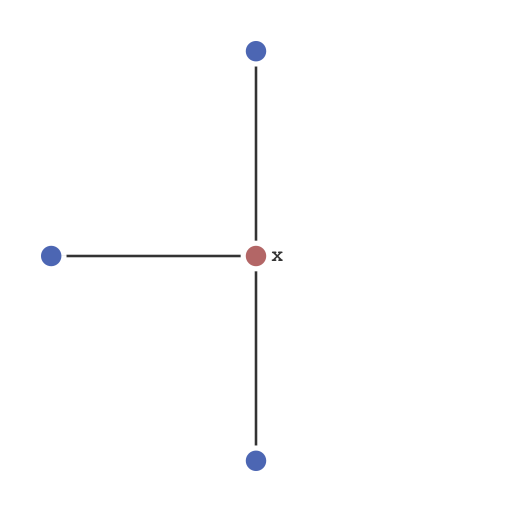
\includegraphics[scale=0.5]{images/brooks/branching_path.png}
                    \caption{Wierzchołek $x$ ma trzech sąsiadów w kolorze $j$}
                \end{figure}
                
            \item Każde dwa $C_{ij}, C_{ik}, k \neq j$ przecinają się tylko w $v_i$ 
                W przeciwnym razie istnieje wierzchołek $x$ w kolorze $i$,
                który ma dwóch sąsiadów w kolorze $j$ i dwóch sąsiadów w kolorze $k$.
                Jak się dobrze policzy to tak jak poprzednio wyjdzie nam, że jakiś kolor jest wolny i możemy zrobić ten sam myk z przekolorowaniem.
                
                \begin{figure}[ht]
                    \centering
                    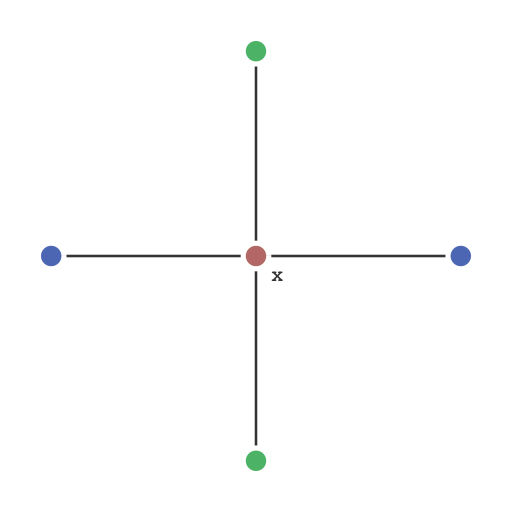
\includegraphics[scale=0.5]{images/brooks/branching_path_three_colors.png}
                    \caption{Wierzchołek $x$ ma dwóch sąsiadów w kolorze $j$ i dwóch w kolorze $k$}
                \end{figure}
                
            \item Istnieje para $v_i, v_j$, która nie jest połączoną krawędzią. 
                W przeciwnym razie wierzchołki $v, v_1, ..., v_\Delta$ tworzą klikę, co jest sprzeczne z założeniem.
                
                Bez straty ogólności powiedzmy, że $v_1$ i $v_2$ nie są połączone krawędzią. Jednak z własności (5) musi istnieć ścieżka między nimi. Niech więc $u$ to będzie pierwszy wierzchołek w kolorze $1$ na ścieżce od $v_2$ do $v_1$.
                
                Teraz dzieje się magia.
                W $C_{23}$ zamieniamy kolory $2$ i $3$ i takie kolorowanie przepuszczamy przez warunki $(2) - (5)$.
                Jeśli w którymś miejscu udało nam się stworzyć dobre kolorowanie to super, a jeśli nie to ups.
                Na szczęście zauważamy teraz fajną rzecz. Otóż wierzchołek $u$ nadal jest połączony ścieżką w kolorach $1$ i $2$ z wierzchołkiem $v_1$, zatem należy do komponentu $C_{12}$, ale z drugiej strony jest połączony krawędzią z wierzchołkiem $v_2$, który ma teraz kolor $3$ zatem należy też do komponentu $C_{13}$.
                W takim razie nowe kolorowanie narusza warunek $(5)$ co już umiemy rozwiązać.
                
                 \begin{figure}[H]
                    \centering
                    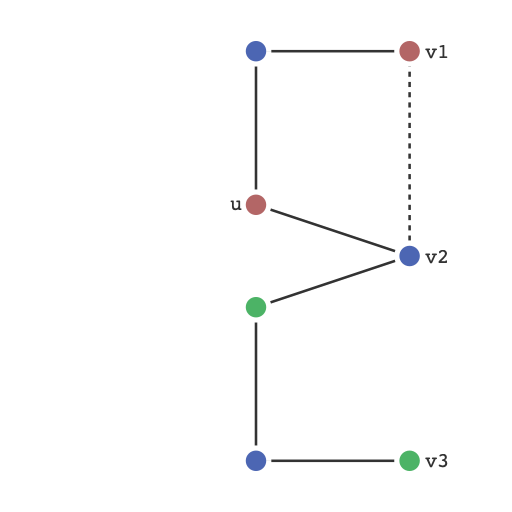
\includegraphics[scale=0.4]{images/brooks/disconnected_before_swap.png}
                    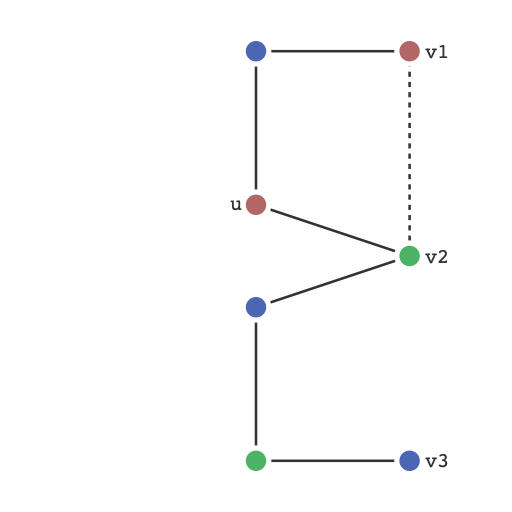
\includegraphics[scale=0.4]{images/brooks/disconnected_after_swap.png}
                    \caption{Wierzchołki $v_1$ i $v_2$ przed i po przekolorowaniu komponentu $C_{23}$}
                \end{figure}
                
                
        \end{enumerate}
        
        To tyle, nie ma więcej warunków, które musimy rozważać. Fajnie.
        
    \end{proof}